% ============================================================================
%  EEE3095S CS Project 2026: Serial Game Server
%  STUDENT REPORT TEMPLATE (IEEE conference format, max 10 pages incl. refs)
% ============================================================================
%
%  How to use this template
%  ------------------------
%  * Red text in [square brackets] is PLACEHOLDER text. Replace every piece of
%    it with your own words. Search the PDF for "[" before you submit.
%  * Grey boxes are GUIDANCE. They tell you what the marker looks for. Leave
%    them on while you write, then switch them off below (\guidancefalse) to
%    check your length against the 10-page limit and before you submit.
%  * Dashed boxes are PLACEHOLDER FIGURES. Replace each with your own diagram
%    (\includegraphics{figures/yourfile.pdf} or TikZ).
%  * Keep the section headings exactly as they are: they are the brief's
%    required headings, in the brief's order, and the marking guide follows
%    them. Add your own subsection headings underneath.
%  * Build:  latexmk -pdf main.tex   (or upload the folder to Overleaf).
% ============================================================================
\documentclass[conference]{IEEEtran}

\usepackage[T1]{fontenc}
\usepackage{cite}
\usepackage{amsmath}
\usepackage{graphicx}
\usepackage{booktabs}
\usepackage{array}
\usepackage{xcolor}
\usepackage{listings}
\usepackage{tikz}
\usepackage{circuitikz}
\usetikzlibrary{automata, positioning, arrows.meta, shapes.geometric}
\usepackage[most]{tcolorbox}
\usepackage[hidelinks]{hyperref}

% ---------------------------------------------------------------- switches --
\newif\ifguidance
\guidancefalse       % guidance off: the report is written, so this shows the true length

% ------------------------------------------------------- template helpers --
\definecolor{phred}{rgb}{0.75,0.08,0.08}
\definecolor{guidebg}{gray}{0.94}
\definecolor{guideframe}{gray}{0.55}

% Placeholder text: replace with your own.
\newcommand{\ph}[1]{\textcolor{phred}{[#1]}}

% Guidance box: what the marker expects. Hidden when \guidancefalse.
\newtcolorbox{guidebox}[1][]{
  breakable, enhanced, colback=guidebg, colframe=guideframe,
  boxrule=0.4pt, arc=1pt, left=3pt, right=3pt, top=2pt, bottom=2pt,
  fontupper=\footnotesize\sffamily, title={#1},
  fonttitle=\footnotesize\sffamily\bfseries, coltitle=black,
  colbacktitle=guidebg!80!gray, before skip=4pt, after skip=6pt}
\newenvironment{guidance}[1][Guidance]
  {\ifguidance\begin{guidebox}[#1]\else\setbox0\vbox\bgroup\fi}
  {\ifguidance\end{guidebox}\else\egroup\fi}

% Placeholder figure: dashed box with a description of what to draw.
% Usage: \figph{<height>}{<what the figure must show>}
\newcommand{\figph}[2]{%
  \begin{tikzpicture}
    \draw[dashed, phred, line width=0.6pt] (0.3pt,0) rectangle (\linewidth-0.3pt,#1);
    \node[text width=0.85\linewidth, align=center, text=phred, font=\footnotesize]
      at (0.5\linewidth,0.5*#1) {#2};
  \end{tikzpicture}}

\newcolumntype{L}[1]{>{\raggedright\arraybackslash}p{#1}}

\lstset{
  basicstyle=\ttfamily\scriptsize, columns=fullflexible, keepspaces=true,
  frame=tb, framerule=0.4pt, commentstyle=\color{gray}\itshape,
  keywordstyle=\bfseries, showstringspaces=false, breaklines=true,
  captionpos=b, float=tbp, floatplacement=tbp,
}
\renewcommand{\lstlistingname}{Listing}

\begin{document}

% ---------------------------------------------------------------- title ----
\title{Serial Game Server: an Authoritative STM32 Tic-Tac-Toe\\
Server with a Thin Python Client}

\author{
\IEEEauthorblockN{Tri Tac Le (LXXTRI004)}
\IEEEauthorblockA{EEE3095S CS Project 2026, Department of Electrical Engineering\\
University of Cape Town}
}

\maketitle

\begin{abstract}
An STM32F051 microcontroller acts as the authoritative referee for a game of
tic-tac-toe while a Python client provides only a view. The board holds the game
state, validates every request and emits exactly one reply per request; the
client enforces no rule, so no modified or faulty client can produce an illegal
position. The two communicate over a line-oriented ASCII protocol on USART1,
carried to the PC by the on-board ST-LINK virtual COM port, with a bounded frame
length, a partial-frame timeout and an optional XOR checksum. The game rules and
the frame parser are plain C with no hardware dependency, so the same sources
build for the microcontroller and for a host simulator and one automated pytest
suite runs against either. Thirty-three tests pass against the host build,
covering every protocol case the brief requires and asserting in each rejection
case that the board is byte-for-byte unchanged.
\end{abstract}

\begin{guidance}[Before you start writing]
\begin{itemize}\setlength\itemsep{0pt}
\item \textbf{Marks} (brief, p.~6): Introduction 10, Protocol 15, Specification
  and design 15, Implementation 15, Game logic and server authority 15,
  Robustness 10, Validation 15, Conclusion 5. Video and Code links are required.
\item \textbf{Limit:} 10 pages \emph{including} references. Switch guidance off
  (\texttt{\textbackslash guidancefalse} in \texttt{main.tex}) to see your true length.
\item \textbf{Write headings that state a finding}, not just a topic, e.g.
  ``Validation runs before any state change'' rather than ``Validation''.
  Keep the section headings below as they are.
\item \textbf{Be specific}: name your mechanisms and give numbers
  (``rejects frames longer than 32 bytes''), not adjectives (``robust'',
  ``efficient'', ``significant'').
\item \textbf{Every figure, table and listing must be referred to and explained
  in the text.} Say what the reader should notice.
\item \textbf{Never present a result you did not measure.} If something is still
  untested on the board, say so.
\end{itemize}
\end{guidance}

\section{Introduction}
\label{sec:intro}

A networked game has to decide where the rules live. If the client enforces
them, every client is part of the trusted computing base and a single modified
or buggy one can corrupt the game. If the server enforces them, the client can
be as simple and as untrusted as you like. This project takes the second
position and pushes it to its limit, as the brief requires~\cite{brief}: the
microcontroller is the only component that may change state, and the PC
application is a view with a mouse attached. The property the design guarantees
is narrow and testable, namely that a rejected request never changes the game
state.

\textbf{The game.} Tic-tac-toe was chosen because its rules are small enough to
implement exactly and to test exhaustively, which puts the interesting work in
the protocol and the authority model rather than in game logic. A nine-cell
board also encodes in nine ASCII characters, so a full board fits in one short
line and the whole state can be sent after every move instead of a delta. That
removes an entire class of client and server disagreeing about state.

\textbf{The GUI library.} Tkinter~\cite{tkinter} was chosen because it ships
with CPython, so the marker needs no package installation to run the client, and
because a three-by-three grid of buttons is exactly what it is good at. It also
has a timer facility that makes it straightforward to keep the window responsive
while a reply is outstanding, which Section~\ref{sec:design} describes. A
heavier toolkit would have added a dependency and bought nothing the application
needs.

\textbf{Design choices.} The rules and the frame parser are plain C with no
hardware abstraction layer (HAL) and no hardware headers, so the same sources
compile for the STM32 and for a host simulator. One file isolates everything
board-specific behind a handful of functions. Messages are framed as single
newline-terminated lines of printable ASCII with a bounded length, which makes
the parser a small finite-state machine (FSM) that can be reasoned about and
fuzzed from a test. The practical consequence is that a rule bug is found in
milliseconds on a laptop rather than on the bench with a debugger.

\textbf{Task allocation.} This project was done individually, so there is no
split of work between two students to report. It was nonetheless organised as if
it were a team: each piece of functionality was developed on its own branch and
merged through a pull request, with the game core, the protocol, the GUI, the
board application and the documentation each landing separately. Reviewing one's
own pull request catches less than a second reader would, but it still forces
the diff to be read once in isolation, keeps unrelated changes from travelling
together, and leaves a history in which each change can be read, and if
necessary reverted, on its own.

\textbf{Structure.} Section~\ref{sec:protocol} defines the message protocol,
since every other part of the system is specified against it.
Section~\ref{sec:design} gives the responsibility split, the server FSM, the
client flow and the hardware connection. Section~\ref{sec:impl} describes how
the firmware is put together, Section~\ref{sec:authority} argues the authority
property from the structure of the code, and Section~\ref{sec:robust} covers
what the parser does with hostile input. Section~\ref{sec:valid} reports the
automated validation and Section~\ref{sec:conclusion} draws conclusions and
names the limitations.

\section{Requirements and Message Protocol}
\label{sec:protocol}

The link carries printable ASCII, one message per line. The client sends a
request and the server answers with exactly one line. The server never speaks
first, so the PC side never has to poll for unsolicited traffic.

\subsection{One newline-terminated line bounds every message}
A message is terminated by \texttt{\textbackslash n}. A
\texttt{\textbackslash r} immediately before it is accepted and discarded, so a
terminal that sends CRLF interoperates without a separate mode. Four limits
bound what the parser will accept:

\begin{itemize}
  \item a frame is at most 64 bytes including the terminator, which leaves 63
        characters of payload; a longer line is discarded up to and including
        the next \texttt{\textbackslash n} and answered
        \texttt{NACK:TOOLONG};
  \item a frame left incomplete for 2000\,ms is cleared, so a client that dies
        mid-line cannot wedge the parser;
  \item bytes outside printable ASCII, that is below \texttt{0x20} or above
        \texttt{0x7E}, are dropped as they arrive rather than buffered;
  \item commands are uppercase, and anything unrecognised is
        \texttt{NACK:BADCMD}.
\end{itemize}

None of these paths can change the game. A rejected, truncated or malformed
request leaves the board, the turn and the game status exactly as they were.

\subsection{The board travels as nine characters}
The board is nine characters, index 0 to 8, row major, where \texttt{.} is an
empty cell and \texttt{X} and \texttt{O} are the players. X always moves first,
so the client derives whose turn it is by counting: equal counts means X to
move. The client therefore holds no authoritative state of its own.

\subsection{Every request has exactly one documented reply}
Table~\ref{tab:protocol} lists the command set. The reader should notice that
every rejection is named: there is no request whose failure produces silence,
which is what lets the client distinguish a refused request from a lost one.

\begin{table}[htbp]
\caption{Command set and responses}
\label{tab:protocol}
\centering
\footnotesize
\begin{tabular}{p{1.8cm}p{3.1cm}p{2.0cm}}
\hline
\textbf{Request} & \textbf{Response} & \textbf{Meaning} \\
\hline
\texttt{CONNECT} & \texttt{OK} & open a session \\
\texttt{NEW} & \texttt{OK:BOARD:.........} & start a game, X to move \\
\texttt{MOVE:<i>} & \texttt{OK:BOARD:<9>} & legal move \\
\texttt{MOVE:<i>} & \texttt{WIN:X}, \texttt{WIN:O}, \texttt{DRAW} & the move ended it \\
\texttt{MOVE:<i>} & \texttt{NACK:RANGE}, \texttt{NACK:OCCUPIED}, \texttt{NACK:NOTURN} & rejected, nothing changed \\
\texttt{STATE} & \texttt{BOARD:<9>} & current board \\
\texttt{RESIGN} & \texttt{OK:GAMEOVER} & forfeit \\
\texttt{DISCONNECT} & \texttt{OK} & end session \\
\hline
\end{tabular}
\end{table}

\subsection{Four departures from the reference protocol}
Each departure closes a failure the reference protocol in the brief leaves
open, and none of them changes a response the brief specifies.

\textbf{\texttt{NACK:TOOLONG}} exists because the reference defines no reply
for an over-length line, which would otherwise leave the client waiting on a
response that never comes.

\textbf{The optional player field on \texttt{MOVE}}, written
\texttt{MOVE:<i>:<p>} where \texttt{<p>} is \texttt{X} or \texttt{O}, lets a
client state whose move it believes it is sending. The server then answers
\texttt{NACK:NOTURN} rather than silently applying the move to the player whose
turn it actually is. Without such a field a single client cannot be out of
turn, so the brief's own out-of-turn requirement would be untestable.

\textbf{\texttt{DISCONNECT} from IDLE} is accepted so that a client
reconnecting after a crash does not have to know what state it left behind. It
is still refused mid-game.

\textbf{An optional \texttt{*HH} checksum suffix} may be appended to any
request. Its scope and its limits are discussed in
Section~\ref{sec:robust}.

\section{Specification and Design}
\label{sec:design}

\subsection{The board decides, the client draws}
Responsibility is split so that the board is the only component that can decide
anything. The STM32 holds the game state, validates every request and emits the
single authoritative reply. The PC client renders what it is told and forwards
clicks; it enforces no rule, which is why a modified or hostile client cannot
produce an illegal position.

Table~\ref{tab:split} sets out who owns what. The pattern to notice is that
every row the client owns is presentation, and every row that could change the
outcome of the game sits on the board.

\begin{table}[htbp]
\caption{Where each decision is taken. Board modules are under \texttt{server/}, client modules under \texttt{client/}.}
\label{tab:split}
\centering
\footnotesize
\begin{tabular}{p{3.7cm}p{1.2cm}p{1.9cm}}
\hline
\textbf{Decision} & \textbf{Owner} & \textbf{Module} \\
\hline
Board contents & board & \texttt{game.c} \\
Whose turn it is & board & \texttt{game.c} \\
Whether a move is legal & board & \texttt{game.c} \\
Win and draw detection & board & \texttt{game.c} \\
Framing and dispatch & board & \texttt{protocol.c} \\
Button and LED meaning & board & \texttt{app.c} \\
When to redraw & client & \texttt{gui.py} \\
What a reply means to the user & client & \texttt{session.py} \\
\hline
\end{tabular}
\end{table}

The firmware is layered so that only one file is hardware-dependent.
\texttt{server/core/} is plain C with no HAL. \texttt{server/stm32/app.c} owns
the button, the LED and the main-loop behaviour but still has no HAL in it, and
\texttt{server/stm32/port\_stm32.c} is the single file that touches registers.
That is what allows the host simulator in \texttt{sim/} to compile the identical
core and application sources.

\subsection{A rejected move returns before the board is written}
Fig.~\ref{fig:fsm} gives the server FSM together with the move-validation
branch. The three states are IDLE, IN\_PROGRESS and GAME\_OVER. IDLE accepts
\texttt{CONNECT} and \texttt{NEW}; IN\_PROGRESS accepts \texttt{MOVE},
\texttt{STATE} and \texttt{RESIGN}; GAME\_OVER accepts \texttt{NEW},
\texttt{STATE} and \texttt{DISCONNECT}. Any command a state does not accept is
answered \texttt{NACK:NOGAME} and changes nothing, which is why those edges are
not drawn individually.

The validation branch is the part worth reading closely. A \texttt{MOVE} passes
three checks in a fixed order, range then turn then occupancy, and each one
exits to its own \texttt{NACK} before the board is touched. Only when all three
pass is the cell written, and only then is the win and draw test run. The
ordering is deliberate: a client that names the wrong player is told so, rather
than being told about a cell it had no business addressing.

\begin{figure*}[t]
\centering
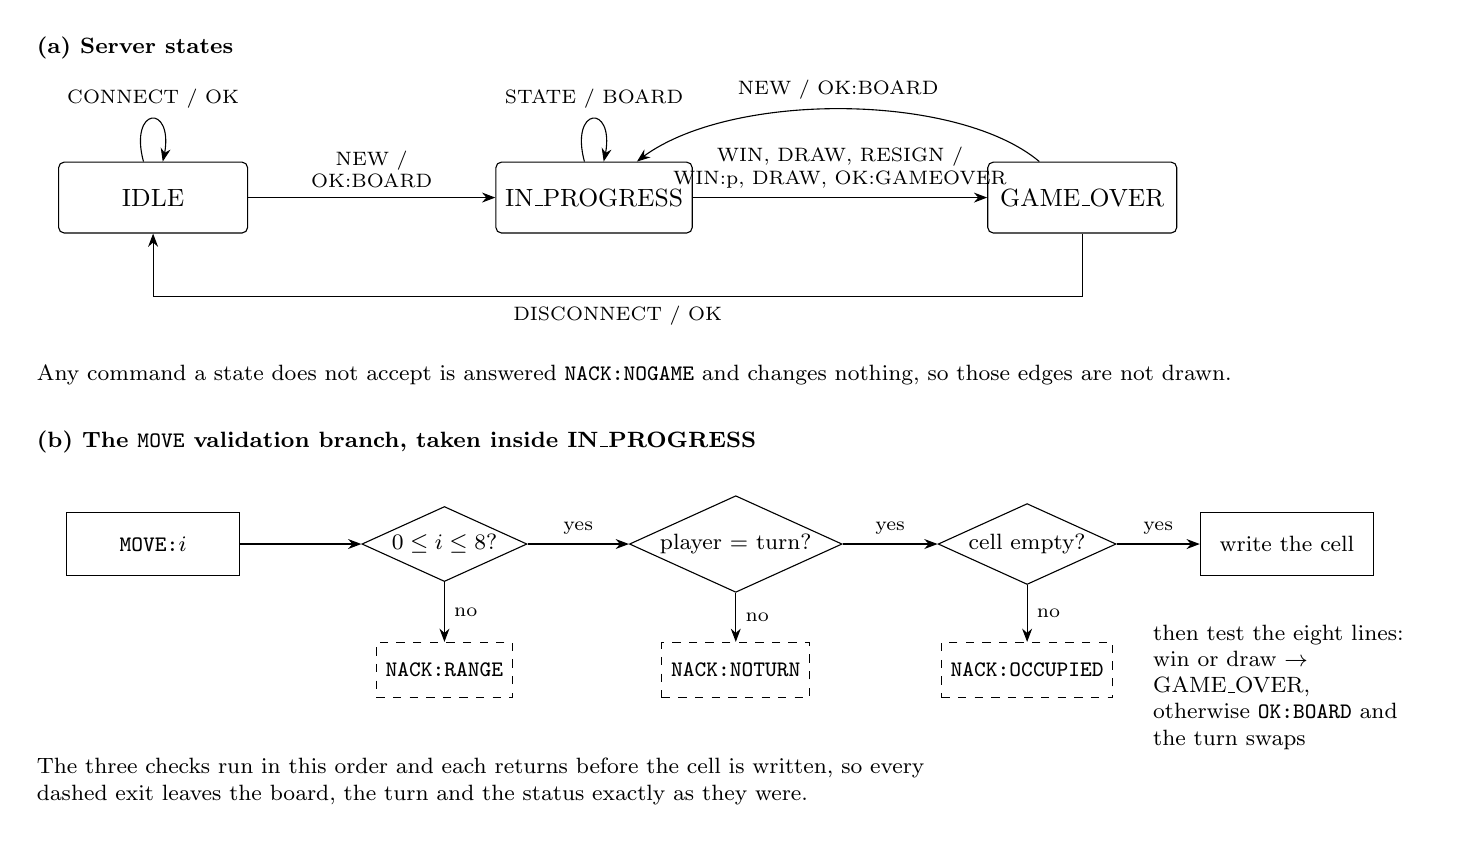
\begin{tikzpicture}[>=Stealth, font=\small,
    st/.style={draw, rounded corners=2pt, minimum width=2.4cm, minimum height=0.9cm},
    chk/.style={draw, diamond, aspect=2.2, inner sep=1pt, font=\footnotesize},
    act/.style={draw, minimum width=2.2cm, minimum height=0.8cm, font=\footnotesize},
    nack/.style={draw, dashed, minimum height=0.7cm, font=\footnotesize},
    note/.style={font=\footnotesize, align=left},
    lbl/.style={font=\scriptsize, align=center}]

  % ---------------- panel (a): the three states
  \node[note, anchor=west, font=\footnotesize\bfseries] at (-1.0,1.9) {(a) Server states};

  \node[st] (idle) at (0.6,0)   {IDLE};
  \node[st] (prog) at (6.2,0)   {IN\_PROGRESS};
  \node[st] (over) at (12.4,0)  {GAME\_OVER};

  \draw[->] (idle) to[loop above] node[lbl, above]{CONNECT / OK} (idle);
  \draw[->] (prog) to[loop above] node[lbl, above]{STATE / BOARD} (prog);
  \draw[->] (idle) -- node[lbl, above]{NEW /\\OK:BOARD} (prog);
  \draw[->] (prog) -- node[lbl, above]{WIN, DRAW, RESIGN /\\WIN:p, DRAW, OK:GAMEOVER} (over);
  \draw[->] (over) to[out=140, in=40, looseness=0.7]
        node[lbl, above]{NEW / OK:BOARD} (prog);
  \draw[->] (over.south) -- ++(0,-0.8) coordinate (d)
        -- node[lbl, below]{DISCONNECT / OK} (d -| idle.south) -- (idle.south);

  \node[note, anchor=north west, text width=15.5cm] at (-1.0,-2.0)
    {Any command a state does not accept is answered \texttt{NACK:NOGAME} and
     changes nothing, so those edges are not drawn.};

  % ---------------- panel (b): what MOVE does inside IN_PROGRESS
  \node[note, anchor=west, font=\footnotesize\bfseries] at (-1.0,-3.1)
    {(b) The \texttt{MOVE} validation branch, taken inside IN\_PROGRESS};

  \node[act] (mv) at (0.6,-4.4) {\texttt{MOVE:}$i$};
  \node[chk] (c1) at (4.3,-4.4) {$0 \le i \le 8$?};
  \node[chk] (c2) at (8.0,-4.4) {player = turn?};
  \node[chk] (c3) at (11.7,-4.4) {cell empty?};
  \node[act] (wr) at (15.0,-4.4) {write the cell};

  \draw[->] (mv) -- (c1);
  \draw[->] (c1) -- node[lbl, above]{yes} (c2);
  \draw[->] (c2) -- node[lbl, above]{yes} (c3);
  \draw[->] (c3) -- node[lbl, above]{yes} (wr);

  \node[nack] (n1) at (4.3,-6.0) {\texttt{NACK:RANGE}};
  \node[nack] (n2) at (8.0,-6.0) {\texttt{NACK:NOTURN}};
  \node[nack] (n3) at (11.7,-6.0) {\texttt{NACK:OCCUPIED}};
  \draw[->] (c1) -- node[lbl, right]{no} (n1);
  \draw[->] (c2) -- node[lbl, right]{no} (n2);
  \draw[->] (c3) -- node[lbl, right]{no} (n3);

  \node[note, anchor=north, text width=3.4cm] at (15.0,-5.3)
    {then test the eight lines:\\
     win or draw $\rightarrow$ GAME\_OVER,\\
     otherwise \texttt{OK:BOARD} and
     the turn swaps};

  \node[note, anchor=north west, text width=12.0cm] at (-1.0,-7.0)
    {The three checks run in this order and each returns before the cell is
     written, so every dashed exit leaves the board, the turn and the status
     exactly as they were.};
\end{tikzpicture}
\caption{Server FSM (a) and the \texttt{MOVE} validation branch (b). The
validation chain sits inside the IN\_PROGRESS state: all three rejections exit
above the single write to the board.}
\label{fig:fsm}
\end{figure*}

\subsection{The client never blocks on the board}
Fig.~\ref{fig:gui} is the client flow. On start it opens the serial port and
sends \texttt{CONNECT}; the New Game button sends \texttt{NEW}; a click on cell
$i$ sends \texttt{MOVE:}$i$ and then repaints from whatever board string comes
back. A \texttt{NACK} is shown verbatim in the status line and the board is left
untouched, because the board the client holds is only ever a copy of the
server's. After a win or a draw the cells are disabled until a new game is
started, and \texttt{STATE} is issued once more so the final position is drawn
from the server rather than from the client's own guess.

The window does not freeze while a reply is outstanding. A daemon reader thread
blocks on the transport and pushes each line it receives onto a
\texttt{queue.Queue}; the Tk main loop drains that queue every 50\,ms through
\texttt{after()} and does all drawing there. A board that never answers
therefore costs a background thread, not the user interface, and the reader
applies its own timeout so a dead link surfaces as a message rather than a hang.

\begin{figure}[htbp]
\centering
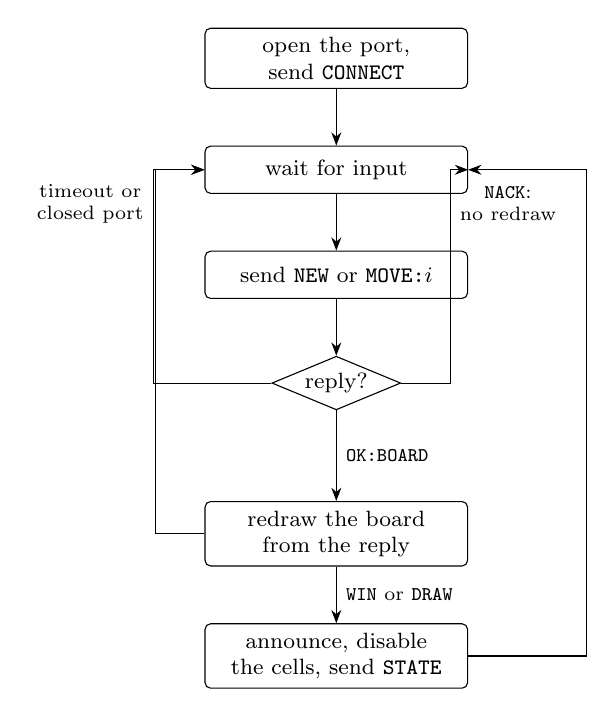
\begin{tikzpicture}[>=Stealth, node distance=0.72cm, font=\footnotesize,
    bx/.style={draw, rounded corners=2pt, text width=3.1cm, align=center,
               minimum height=0.6cm},
    df/.style={draw, diamond, aspect=2.4, inner sep=1pt, align=center},
    lbl/.style={font=\scriptsize, align=center}]

  \node[bx] (start) {open the port, send \texttt{CONNECT}};
  \node[bx, below=of start] (wait) {wait for input};
  \node[bx, below=of wait] (send) {send \texttt{NEW} or \texttt{MOVE:}$i$};
  \node[df, below=of send] (rep) {reply?};
  \node[bx, below=1.15cm of rep] (draw) {redraw the board from the reply};
  \node[bx, below=of draw] (over) {announce, disable the cells, send \texttt{STATE}};

  \draw[->] (start) -- (wait);
  \draw[->] (wait) -- (send);
  \draw[->] (send) -- (rep);
  \draw[->] (rep) -- node[lbl, right]{\texttt{OK:BOARD}} (draw);
  \draw[->] (draw) -- node[lbl, right]{\texttt{WIN} or \texttt{DRAW}} (over);

  % right, inner: a NACK goes straight back to waiting
  \draw[->] (rep.east) -- ++(0.62,0) |- node[lbl, right, pos=0.42]
    {\texttt{NACK}:\\no redraw} (wait.east);
  % right, outer: a finished game waits for a new one
  \draw[->] (over.east) -- ++(1.5,0) |- (wait.east);
  % left, inner: an ordinary redraw returns to waiting
  \draw[->] (draw.west) -- ++(-0.62,0) |- (wait.west);
  % left, outer: a timeout or a closed port
  \draw[->] (rep.west) -- ++(-1.5,0) |- node[lbl, left, pos=0.42]
    {timeout or\\closed port} (wait.west);
\end{tikzpicture}
\caption{Client flow. Every redraw is driven by a server reply; a
\texttt{NACK} and a timeout both return to waiting without touching the board.}
\label{fig:gui}
\end{figure}

\subsection{One USB cable carries both the flashing and the link}
Fig.~\ref{fig:circuit} shows the connection. USART1 is PA9 for transmit and
PA10 for receive, and on this board both are wired on-board to the ST-LINK,
which also presents a USB virtual COM port. One cable therefore does both jobs
and no external USB-to-UART converter is involved, which is what the course
confirmed on 5 October 2026. The link runs at 115\,200 baud, 8 data bits, no
parity, one stop bit, no flow control, and the PC side appears as
\texttt{/dev/ttyACM0} on Linux.

Button0 is on PA0 behind a pull-up, so a press reads low, and the application
debounces it over 20\,ms and then feeds a synthetic \texttt{NEW} through the
server rather than resetting the game behind the protocol's back. LED0 is on
PB0 and reports whose turn it is: solid while X is to move, off while O is, and
blinking at 400\,ms whenever no game is running, which covers both the idle
board before the first game and a finished one. A glance at the board therefore
says whose turn it is, or that there is no turn to take, without looking at the
GUI.

\begin{figure}[htbp]
\centering
\begin{circuitikz}[american, scale=0.74, transform shape,
                   every node/.append style={font=\footnotesize}]
  \node[draw, minimum width=1.2cm, minimum height=0.9cm] (pc)  at (0,0)    {PC};
  \node[draw, minimum width=2.1cm, minimum height=0.9cm] (stl) at (2.9,0)  {ST-LINK VCP};
  \node[draw, minimum width=2.0cm, minimum height=2.6cm] (mcu) at (7.2,-0.7) {STM32F051};

  \draw (pc.east) -- node[above, font=\scriptsize]{USB} (stl.west);

  % USART1 to the on-board ST-LINK
  \draw[->] ([yshift=0.2cm]stl.east) -- node[above, font=\scriptsize]{PA9 TX}
        ([yshift=0.75cm]mcu.west);
  \draw[<-] ([yshift=-0.2cm]stl.east) -- node[below, font=\scriptsize]{PA10 RX}
        ([yshift=0.25cm]mcu.west);

  % Button0 on PA0, active low
  \draw ([yshift=-0.7cm]mcu.west) -- ++(-1.5,0) coordinate (b)
        node[above, pos=0.55, font=\scriptsize]{PA0};
  \draw (b) to[push button, l_={\scriptsize Button0}] ++(0,-1.3) node[ground]{};

  % LED0 on PB0
  \draw ([yshift=0.5cm]mcu.east) -- ++(1.2,0) coordinate (d)
        node[above, pos=0.55, font=\scriptsize]{PB0};
  \draw (d) to[R, l^={\scriptsize $R_s$}] ++(0,-1.1)
        to[leD, l^={\scriptsize LED0}] ++(0,-1.1) node[ground]{};
\end{circuitikz}
\caption{UART path and board I/O. One USB cable carries both the programming
interface and the virtual COM port that USART1 is wired to. Button0 is active
low and starts a new game; LED0 is solid while X is to move, off while O is,
and blinks at 400\,ms whenever no game is running.}
\label{fig:circuit}
\end{figure}

\section{Implementation}
\label{sec:impl}

\subsection{The receive path cannot block}
Bytes arrive one at a time in the USART1 receive interrupt and are appended to
a line buffer. The interrupt does no parsing: it tests for the terminator, and
only when a complete line is present does it hand that line to the protocol
layer. Nothing in the receive path waits on anything, so a client that stops
mid-message costs the board nothing but a buffer that the 2000\,ms timeout will
later clear. An overrun is cleared and the byte dropped rather than left to
wedge the receiver, because the parser already recovers at the next newline.

\subsection{Three checks, one write}
\texttt{game\_move()} tests range, then turn, then occupancy, and each check
returns before the board is touched:

\begin{verbatim}
if (index < 0 || index >= GAME_CELLS)
    return MOVE_ERR_RANGE;
if (player != 0 && player != g->turn)
    return MOVE_ERR_NOTURN;
if (g->cells[index] != '.')
    return MOVE_ERR_OCCUPIED;

g->cells[index] = g->turn;
\end{verbatim}

There is exactly one assignment to \texttt{g->cells}, and all three rejection
paths return above it. That structure, rather than an inspection of every path,
is what makes the authority argument in Section~\ref{sec:authority} hold.

\subsection{One core, two targets}
\texttt{server/core/} contains the rules and the frame parser in plain C with
no HAL and no hardware headers. \texttt{server/stm32/port\_stm32.c} is the only
file that knows about the board, and it provides the functions declared in
\texttt{port.h}: bring up the USART, service its interrupt, transmit a line,
drive the LED, read the button and report a millisecond tick. The same core
therefore builds unchanged for the board and for the host simulator in
\texttt{sim/}, so a rule bug is found on a laptop in milliseconds rather than
on the bench.

The board project in \texttt{board/} reaches the shared sources through linked
folders rather than copying them, so there is one copy of every file and the
two builds cannot drift apart. GPIO goes through the HAL because the GPIO
driver ships with the course project, while USART1 is configured from registers
against the reference manual~\cite{rm0091} because the vendored HAL has no UART
driver at all. At 48\,MHz and 115\,200 baud with oversampling by 16 the baud
rate register is the divisor itself, so \texttt{BRR} is 417, which gives
115\,107 baud and an error of 0.08\,per cent.

The release build occupies 4984 bytes of flash and 2720 bytes of RAM, against
the 32\,kB of flash and 8\,kB of RAM that the linker script reserves. The board
used here in fact reports 64\,kB of flash and 8\,kB of RAM when probed, so
neither figure is close to a constraint either way.

\section{Game Logic and Server Authority}
\label{sec:authority}

Turn control is held entirely on the board. \texttt{g->turn} is advanced only
after a move has been accepted and found not to end the game, so a rejected
request cannot hand the turn to the other player either.

A win is detected by testing the eight lines, three rows, three columns and two
diagonals, for three identical marks immediately after the cell is written; a
draw is the case where the board is full and no line was won. Both set
GAME\_OVER, after which only \texttt{NEW}, \texttt{STATE} and
\texttt{DISCONNECT} are accepted.

The authority claim is that \textbf{no rejected request can change state}, and
it rests on the structure quoted in Section~\ref{sec:impl} rather than on
inspection of every path: the three validation checks all return before the
sole write to the board. The claim is deliberately narrow enough to test from
the outside, and Section~\ref{sec:valid} describes how the suite asserts it by
reading the board with \texttt{STATE}, issuing a request expected to fail, and
reading it again.

The client is given no way to acquire authority. It holds no copy of the rules,
it derives whose turn it is only for display, and every redraw is driven by a
reply rather than by a local prediction. Replacing the client with a hostile one
therefore changes nothing about what positions are reachable: the worst a
modified client can do is send a request the server refuses.

\section{Protocol Robustness and Integrity}
\label{sec:robust}

\subsection{The parser assumes the line is hostile}
Over-length input is bounded by the 64-byte frame limit and answered
\texttt{NACK:TOOLONG}, with the remainder of the offending line discarded so
that its tail is not then parsed as a fresh command. Non-printable bytes are
dropped as they arrive rather than buffered. A partial frame is abandoned after
2000\,ms, so a client that dies mid-line releases the parser without
intervention. A bare newline is ignored rather than answered.

An unrecognised command is \texttt{NACK:BADCMD}. The index on a \texttt{MOVE}
is exactly one digit, so \texttt{MOVE:9} is a well-formed request for a cell
that does not exist and is answered \texttt{NACK:RANGE}, while
\texttt{MOVE:99}, \texttt{MOVE:-1} and \texttt{MOVE:} are malformed and are
answered \texttt{NACK:BADCMD}. The two are distinguished because they indicate
different client faults, and both were confirmed against the board.

Every rejection is explicit. The server never answers silence, so a client can
always distinguish a refused request from a lost one by timeout alone.

\subsection{The checksum detects corruption, not forgery}
An optional \texttt{*HH} suffix carries an XOR of every byte before the
\texttt{*}, as two hex digits in either case. When the suffix is absent the
message is accepted unchecked; when it is present and wrong the message is
answered \texttt{NACK:BADCRC} and dropped.

It detects single-byte corruption and most burst corruption on the wire, which
is what a short UART link is likely to suffer. It is not a cryptographic check:
an XOR is trivially forgeable, it cannot detect a transposition of two bytes,
and it offers nothing against replay or against a client that is simply lying
about whose turn it is. Integrity against a hostile client is provided by server
authority, as argued in Section~\ref{sec:authority}, and not by the checksum.

\section{Validation}
\label{sec:valid}

\subsection{One suite, two targets}
The automated suite is written with pytest~\cite{pytest}. It drives the comms
interface with no human interaction and runs against two targets from the same
test files. By default it starts the host
simulator and speaks the protocol over its standard input and output; given
\texttt{-{}-port} it opens a serial port through pyserial~\cite{pyserial} and
speaks to the flashed board instead. The fixture that performs that substitution is the only thing that
differs between the two runs, so a case that passes on the host is the same case
on the board.

\subsection{Thirty-three cases pass on the host build}
The following is a run on the host simulator, on a PC, with no board attached:

{\footnotesize
\begin{verbatim}
$ make -C sim && python -m pytest tests -q
.................................    [100%]
33 passed in 0.10s
\end{verbatim}}

Table~\ref{tab:tests} maps each case the brief requires onto the test that
covers it. The suite is a regression check rather than a demonstration: every
run either reproduces the protocol exactly or fails.

The cases fall into three groups. The first confirms the happy path, that
\texttt{CONNECT} is answered and \texttt{NEW} produces an empty board. The
second confirms that a legal move changes the board \emph{exactly} as expected,
comparing the whole nine-character string rather than the single cell, so a move
that corrupted a neighbouring cell would fail. The third is the authority group:
each test reads the board, issues a request that must be refused, and reads the
board again, asserting the two are identical. Seven of the tests are of that
third kind, which is the property Section~\ref{sec:authority} claims.

Beyond the required cases the suite also covers the robustness paths: an
over-length frame and the recovery after it, non-printable bytes, a request
split across two writes and reassembled, a CRLF terminator, and a checksum that
is correct and one that is not.

\subsection{Results from the board}
\ph{Run the same suite against the flashed board with
\texttt{python -m pytest tests -{}-port /dev/ttyACM0 -q} and paste that output
here, labelled as the board run so it is not confused with the host run above.
Note that pyserial must be installed first.}

\ph{Add the two GUI screenshots to \texttt{figures/} and refer to them here:
one mid-game showing a rejected move and its reason in the status line, and one
after a win showing the cells disabled. Say what the reader should notice in
each.}

Nothing in this section claims a measurement that has not been taken: the
figures quoted above are from the host build, and the board run is recorded
separately once it has been performed.

\begin{table}[htbp]
\caption{Required test cases and where they are covered. Test names are shown without their \texttt{test\_} prefix.}
\label{tab:tests}
\centering
\footnotesize
\begin{tabular}{p{4.0cm}p{3.3cm}}
\hline
\textbf{Required by the brief} & \textbf{Test} \\
\hline
CONNECT returns OK & \texttt{connect\_\allowbreak returns\_\allowbreak ok} \\
NEW returns an empty board & \texttt{new\_\allowbreak returns\_\allowbreak an\_\allowbreak empty\_\allowbreak board} \\
A legal move changes the board & \texttt{a\_\allowbreak legal\_\allowbreak move\_\allowbreak changes\_\allowbreak the\_\allowbreak board\_\allowbreak exactly} \\
Occupied cell rejected, board unchanged & \texttt{occupied\_\allowbreak cell\_\allowbreak is\_\allowbreak rejected\_\allowbreak and\_\allowbreak nothing\_\allowbreak changes} \\
Out of range rejected & \texttt{out\_\allowbreak of\_\allowbreak range\_\allowbreak is\_\allowbreak rejected} \\
Move after game over refused & \texttt{moves\_\allowbreak after\_\allowbreak game\_\allowbreak over\_\allowbreak are\_\allowbreak refused} \\
Scripted win and draw & \texttt{a\_\allowbreak win\_\allowbreak is\_\allowbreak detected}, \texttt{a\_\allowbreak draw\_\allowbreak is\_\allowbreak detected} \\
\hline
\end{tabular}
\end{table}

\section{Conclusion}
\label{sec:conclusion}

The system works and the design decision at the centre of it holds up. Keeping
the microcontroller authoritative made the client trivial to write and
impossible to cheat with, and the tests demonstrate the property directly rather
than arguing for it: every rejection case reads the board, issues a request that
must fail, and asserts the board is unchanged.

The decision with the largest practical payoff was separating the rules from the
hardware. Because \texttt{server/core/} has no HAL in it, the same sources run
on a host simulator, which meant the protocol and the game logic were finished
and tested before the board was involved at all. On a project with a fixed
deadline that converts bench time into laptop time, which is the cheaper of the
two.

\textbf{Limitations.} The server holds one game and one session, so it cannot
serve two clients at once; the state machine would need a session table rather
than a single \texttt{game\_t} to do so. Frames are capped at 64 bytes, which is
comfortable for this protocol but would need revisiting for a larger board. The
optional checksum detects corruption on the wire but is an XOR, so it is not
forgery-resistant, and integrity against a hostile client rests on server
authority instead. Transmission from the board is blocking with a timeout, which
is acceptable at 115\,200 baud and one short line per request but would not
scale to a chattier protocol.

\textbf{Further work.} The most natural extension is the AI opponent listed
among the bonus features, which fits the architecture without changing the
protocol: the server already owns the state, so it can generate a reply move
after a client move, and the existing suite could assert that it never plays
illegally. Beyond that, a session table would allow multiple concurrent games,
and a larger board would mostly be a matter of relaxing the frame limit and the
index parser.

\section{Video}
\label{sec:video}

The demonstration video is available at
\url{https://www.youtube.com/watch?v=JrKrHBp4w70}. It is unlisted rather than
private, so the link opens without a YouTube account.

It shows, in order: opening the port and connecting; a new game; a legal move
and the redraw that follows it; a rejected move with its reason in the status
line and the board visibly unchanged; a win, after which the cells are disabled;
the on-board button starting a fresh game; the LED reporting whose turn it is;
and a clean disconnect. Both the board and the screen are in frame.

\section{Code}
\label{sec:code}

The source code is at \url{https://github.com/TriTacLe/EEE3095S-project}. The
repository is public, so the link opens without a GitHub account.

The repository holds the board project in \texttt{board/}, the hardware-free
game core and board application in \texttt{server/}, the Tkinter client in
\texttt{client/}, the host simulator in \texttt{sim/} and the pytest harness in
\texttt{tests/}. Setup, build, flash, run and test instructions are in the
top-level \texttt{README.md}, with the board-specific steps in
\texttt{board/README.md}.


\bibliographystyle{IEEEtran}
\bibliography{refs}

\end{document}
